\section{Proviamo a fissare una dimensione}
Come abbiamo visto in precedenza, l'approccio di Hough prevede un tensore a quattro dimensioni. Per aggirare parzialmente questo problema, possiamo fissare un parametro della curva, come ad esempio $d$ (l'ampiezza), in modo tale da ridurre a tre il numero delle dimensioni del tensore.\par
Come si può osservare nello \hyperref[lst:ostinelli_Tensore3]{pseudocodice} a pagina seguente, questa soluzione è abbastanza semplice da implementare e permette di risolvere alcuni problemi.\par
In primo luogo, risolviamo parzialmente il problema relativo all'impiego di memoria, poiché abbiamo diminuito il numero di dimensioni, quindi abbiamo sensibilmente meno valori da memorizzare.\par
Per quanto riguarda la difficoltà di rendere intelleggibile una struttura del genere, ci sono degli escamotage che permettono la visualizzazione in maniera chiara delle quattro dimensioni, facendo uso dei colori come nell'esempio seguente.

\begin{figure}[h]
    \centering
    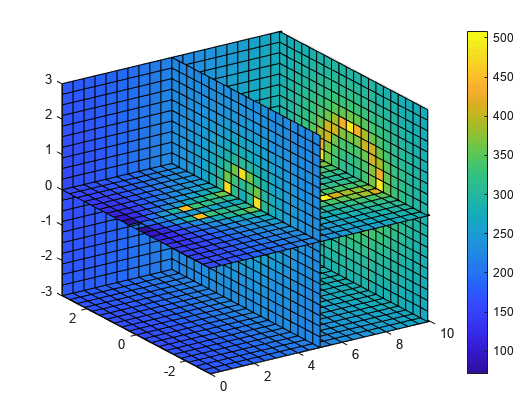
\includegraphics[width=0.8\textwidth]{immagini/altro/volume4D.png}
    \caption{Esempio di Visualizzazione 4D da MathWorks \cite{mathworks}}
\end{figure}

\newpage
\lstinputlisting[
    style=matlabStyle,
    caption={Pseudocodice per la trasformata di Hough per curve ad S con d fissato},
    label={lst:ostinelli_Tensore3}
]{codici/Ostinelli_Tensore3.m}
\newpage

\subsection{Analizziamo qualche esempio}
Come accennato prima, per analizzare gli esempi, usiamo una struttura in cui la quarta dimensione è rappresentata dal colore.\par
Per rendere comprensibile tale struttura usiamo tre piani di taglio, uno per ogni dimensione del tensore, per andare a verificare i colori all'interno della zona d'interesse: $c,\ b$ ed $a$, rappresentati rispettivamente da $y,\ x$ e $z$.\par
Nel \hyperref[fig:4D_ostinelli_1]{primo esempio} è possibile vedere come la curva venga identificata al centro. Dal punto di vista isometrico, notiamo che grazie al parametro $a$, si crea sul piano verticale, una sorta di parabola che identifica la presenza di asintoti abbastanza lunghi.\par
Infatti, nel \hyperref[fig:4D_ostinelli_2]{secondo esempio}, dove la stessa curva ha gli asintoti tagliati, notiamo una parabola sul piano verticale più stretta.\par
Nel \hyperref[fig:4D_ostinelli_3]{terzo} e \hyperref[fig:4D_ostinelli_4]{quarto esempio}, notiamo come sia precisa l'identificazione della posizione del centro della curva. I piani infatti sono stati collocati esattamente nel punto di massimo assoluto del tensore.\par
Nel \hyperref[fig:4D_ostinelli_5]{quinto esempio}, invece, è possibile osservare la maggior larghezza della parabola sull'asse verticale, dovuta all'importante ampiezza della curva stessa. Infatti la curva va a posizionarsi parzialmente su una serie di parametrizzazioni al variare di $a$.\par
Infine, il \hyperref[fig:4D_ostinelli_6]{sesto esempio} verifica la presenza di entrambe le curve singolarmente. Per comodità di lettura, gli assi sono stati posizionati su una delle due sigmoidi. Dopo vedremo che questa precisione sia dovuta al fatto che il parametro $d$ sia fissato.


\foreach \i in {1,...,6} {
    \newpage
    \subsubsection{Esempio in 4 dimensioni n.\i}
    \vfill
    \begin{center}
    \begin{figure}[H]
        \label{fig:4D_ostinelli_\i}
        \centering
        \begin{subfigure}{0.40\textwidth}
            \centering
            \includegraphics[width=\linewidth, frame]{immagini/sintetiche/\i.png}
            \caption*{Input}
        \end{subfigure}

        \vspace{20pt}
        
        \begin{subfigure}{0.43\textwidth}
                \centering
                \includegraphics[width=\linewidth, frame]{immagini/4D_risultati_sintetiche/\i_isometrica.png}
                \caption*{Isometrica}
            \end{subfigure}
            
        \vspace{20pt}
        
        \begin{subfigure}{0.43\textwidth}
                \centering
                \includegraphics[width=\linewidth, frame]{immagini/4D_risultati_sintetiche/\i_sotto.png}
                \caption*{Sotto}
            \end{subfigure}
    \end{figure}
    \end{center}
}
